% !TEX root = recommending-interesting-writing.tex
\section{Evaluation}
\label{sec:experiments}

We conduct an offline empirical study of the performance of \acrlong{rfs} to assess its performance as a recommendation model. Then we qualitatively evaluate the visual interface to study whether the explanation-aware, controllable interface enabled by \gls{rfs} can help make editors at The Browser make better decisions.

\paragraph{Data Collection and Preprocessing.} For positive examples, we use the historical set of articles curated by editors at The Browser. We augment the training data with articles selected by the editors of other curation services, and treat all positively-labeled examples curated by editors as data from a single user due to a paucity of data. We use articles from news websites as examples with negative labels, and collect additional articles with negative labels from websites most-featured by the editors to mimic the editorial process of reading a large swath of articles in a feed and distilling an article list to a select few. For preprocessing the data we use the tokenizer released by \textcite{devlin2019bert:} and discard words not recognized by the tokenizer. This procedure results in a dictionary with $30$k words, and $646$k datapoints with $27$k positive labels.

\paragraph{Metrics} Performance of the recommendation models is assessed with recall, and $15\%$ of the datapoints are held out for the validation and test sets respectively.

\paragraph{Experimental setup: RankFromSets} We cross-validate using the RMSProp optimizer~\parencite{tieleman2012lecture} with a momentum of $0.9$ and grid search over learning rates of $\{10^{-2}, 10^{-3}, 10^{-4}, 10^{-5}\}$, whether or not to initialize from pre-trained \acrshort{bert} embeddings~\parencite{wolf2019huggingfaces}, and embedding sizes of $\{10,25,50, 100, 500, 1000\}$. This model is trained on an NVIDIA Tesla P100 GPU.

\paragraph{Experimental setup: \acrshort{bert}} To fine-tune \acrshort{bert}, we use the AdamW optimizer with a linear learning rate scheduler and warmup steps, with a batch size of $32$ and maximum input length of $512$ as in \textcite{devlin2019bert:} and \textcite{wolf2019huggingfaces}. A grid search is performed over learning rates of $\{2, 3, 4, 5\} \times 10^{-5}$, warmup steps of $\{10^2, 10^3, 10^4\}$, and total training steps of $\{10^2, 10^3, 10^4, 10^5\} \times 5$. The model is trained on an NVIDIA Tesla V100 GPU.

The best-performing model of \gls{rfs} is selected for deployment, and recall is evaluated on the test set, after using early stopping according to validation recall. The results are shown in \Cref{tab:recall}, and \gls{rfs} outperforms \acrshort{bert} by $14\%$. Further, \gls{rfs} achieves better performance ten times faster than \acrshort{bert}, as shown in \Cref{fig:training-recall}. In a test to measure the speed of recommending $10^4$ held-out articles, \gls{rfs} ranked all articles in $120$ ms on a CPU, while \acrshort{bert} took $4$ m $54$ s to rank the articles on an NVIDIA Tesla V100 GPU. This represents a 2000-fold improvement in speed, which is beneficial for the controllable visual interface that requires \Cref{eq:inner-product-control} to be quickly computed in response to user input.

\begin{figure}[!tb]
  \centering
  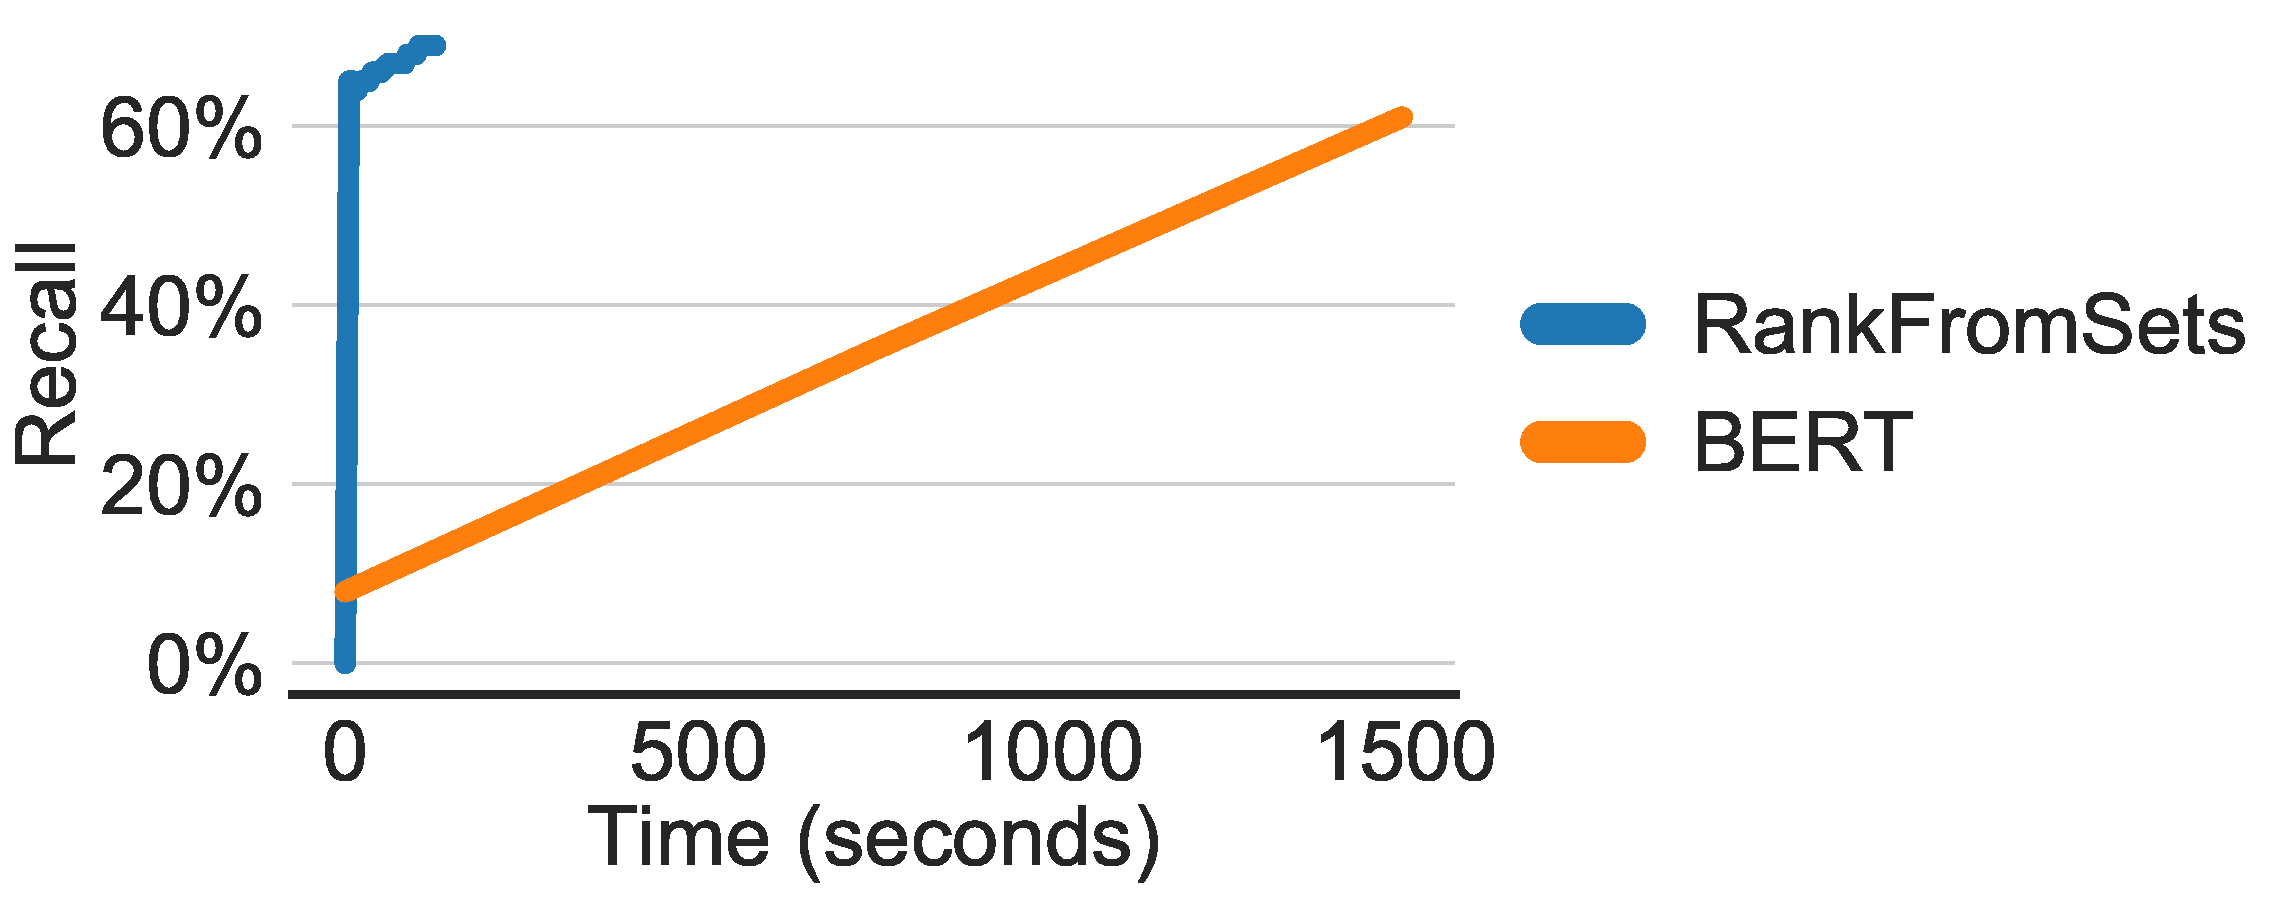
\includegraphics[width=0.95\linewidth]{fig/training-recall}
  \caption{\acrlong{rfs} outperforms models based on word embeddings
    permutation-marginalized recurrent neural networks (denoted by LSTM) on meal
    recommendation. The recommendation models are trained on data from a food
    tracking app as described in \Cref{sec:experiments_meals} and are evaluated
    using the sampled recall metric, \Cref{eq:sampled-recall}. The inner
    product, neural network, and residual regression functions for \acrlong{rfs}
    are in \Cref{eqn:rankfromsets,eqn:neural-network,eqn:residual}.}
  \label{fig:training-recall}
\end{figure}
% !TEX root = ../recommending-interesting-writing.tex
\begin{table}[tb]
\centering
\begin{tabular}{lSS}
\toprule
Recommendation Model & \multicolumn{1}{c}{Recall @ 1000 (\%)}
\\
\midrule
\acrlong{rfs} &  \bfseries 53.1\\
\acrshort{bert} & 46.6 \\
\bottomrule
\end{tabular}
% BERT 466/1000
% rankfromsets 531/1000
% \vspace{1ex}
\caption{\gls{rfs} outperforms \acrshort{bert} in an offline evaluation, on a task of predicting which articles editors at The Browser would feature based on words in the articles.}
\label{tab:recall}
\end{table}

\paragraph{Qualitative Evaluation} In a user study, editors at The Browser provided feedback that they used the visual interface to choose articles, and found this to be an improved workflow. The control over recommendations, and explanation-aware visual interface provided by \gls{rfs} helped elicit bugs in data collection (such as foreign language sources, or fiction writing) and provides an enjoyable user experience.